\documentclass[12pt,a4paper]{article}
\usepackage{geometry}
\geometry{a4paper, margin=1in}
\usepackage{fontspec}
\usepackage{hyperref}
\usepackage{graphicx}
\usepackage{booktabs}
\usepackage{longtable}
\usepackage{array}
\usepackage{xcolor}
\usepackage{setspace}
\usepackage{caption}
\usepackage{titlesec}
\usepackage{float}
\usepackage{placeins}
\usepackage{listings}

\lstset{
    basicstyle=\ttfamily,
    breaklines=true,
    columns=fullflexible,
    keepspaces=true,
    upquote=true,
    literate={-}{-}1
}

% APA-inspired settings
\setstretch{1.25}
\setlength{\parindent}{0.5in}

% Font Policy: Times New Roman for body, serif for title
\setmainfont{Times New Roman}
\setsansfont{Times New Roman}

\title{Technical Report \\ \large TPT Data Explorers 2026}
\author{Data Explorers Team}
\date{\today}

\begin{document}

\begin{titlepage}
    \centering
    \vspace*{2in}
    {\Huge \bfseries Technical Report \par}
    \vspace{0.5in}
    {\Large \bfseries TPT Data Explorers 2026 \par}
    \vspace{1.5in}
    {\large Data Explorers Team \par}
    \vspace{0.5in}
    {\large \today \par}
    \vfill
\end{titlepage}

\newpage
\begin{center}
\textbf{Abstract}
\end{center}
\addcontentsline{toc}{section}{Abstract}

The TPT Data Explorers 2026 project addresses crucial supply chain management and dealer behavior analysis challenges for Thong Nhat Bike. Amidst market volatility and a severe 9-month data gap spanning from April 2025 to December 2025, this technical report presents three core analytical tracks intended to stabilize the business forecasting baseline. First, the Product Demand Forecasting track for Q2 2026 navigates the March 2026 Demand Shock to optimize procurement. Second, an in-depth trend analysis of product colors and variants provides actionable inventory insights. Third, the prediction of dealer ordering behavior leverages RFM B2B segmentation coupled with classification modeling. A hybrid approach utilizing Group-Share Proportional methodologies alongside experimental Machine Learning sets provides a reproducible operational baseline, while strictly acknowledging systemic constraints due to historical data sparsity.

\vspace{0.5in}
\noindent \textbf{Keywords:} Supply Chain, Demand Forecasting, RFM B2B, Machine Learning, Inventory Optimization.
\FloatBarrier


\newpage
\tableofcontents
\newpage

\section{Introduction}
Thong Nhat Bike faces an immediate operational need to systematically forecast the ordering behavior of its diverse B2B dealer network. Accurate forecasting not only optimizes working capital tied up in inventory but also directs targeted customer care campaigns efficiently. A successful forecasting system must delicately balance algorithmic sensitivity with clear business interpretability.

The project structurally focuses on three primary tracks. Track 1 forecasts volume allocation by SKU to preempt supply chain disruptions. Track 2 analyzes underlying color trends, acting as a critical attribute affecting stock turnover rates. Track 3 systematically scores and ranks dealer priorities to support customer care resource allocation, leveraging behavioral RFM modeling to personalize engagement strategies.
\FloatBarrier

\section{System Architecture}
The system is designed with a strict modular approach, ensuring individual components can evolve independently. The Database Layer utilizes PostgreSQL as the central reliable storage mechanism. Ingestion processes handle both historical data seeds and automated pipelines that extract unstructured transactions from emails and PDFs.

Figure \ref{fig:arch} illustrates the holistic Data Flow. Extracted data undergoes a robust ETL layer to patch structural and historical inconsistencies. The Feature Store systematically transforms transactional records into continuous Time-series Panels. All forecasting artifacts are eventually exported as CSV datasets and accessible SQL Views.

\begin{figure}[H]
\centering
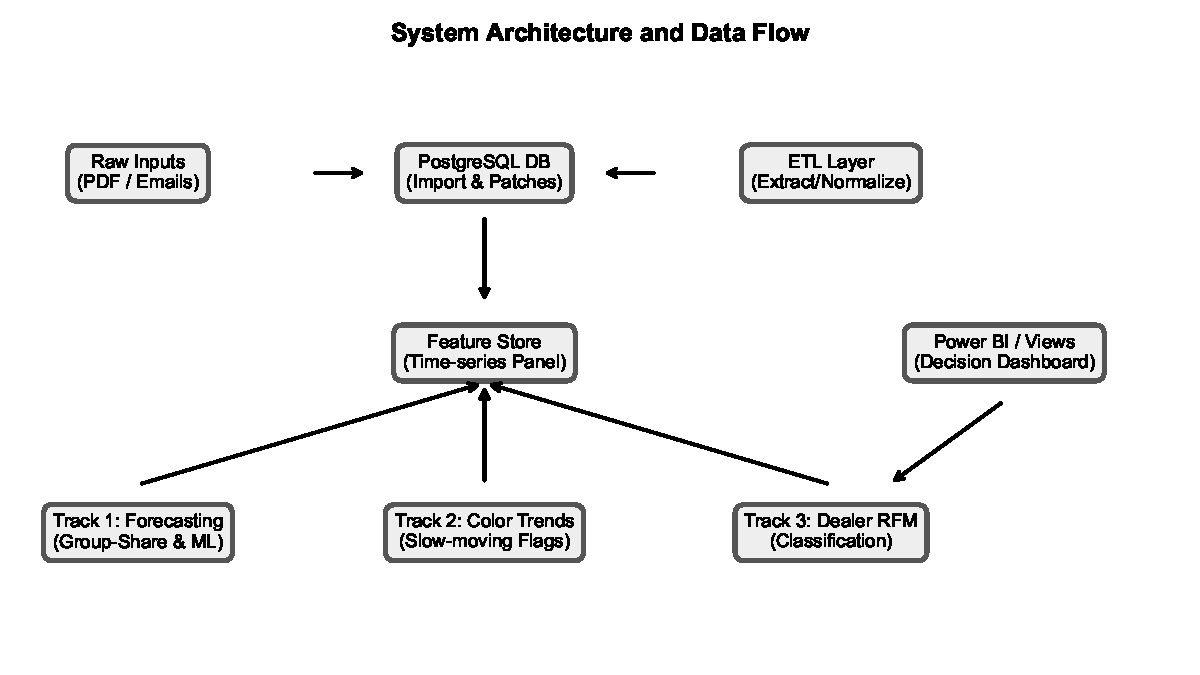
\includegraphics[width=0.85\textwidth]{../figures/en/architecture.pdf}
\caption{System Architecture and Data Flow Diagram}
\label{fig:arch}
\end{figure}

The clear separation of concerns inherent in this layered architecture supports maintainability and codebase reusability for future cyclical updates.
\FloatBarrier

\section{Database and ETL Pipeline}
Raw data processing is split into historical seeding and real-time ingestion protocols. Table \ref{tab:pipeline} lists the primary scripts orchestrating these operations and their specific roles within the ecosystem.

\begin{table}[H]
\centering
\small
\caption{Pipeline Components and ETL Scripts}
\label{tab:pipeline}
\resizebox{\linewidth}{!}{
\begin{tabular}{lll}
\toprule
\textbf{Component} & \textbf{Script Alias} & \textbf{Role} \\
\midrule
Database Init & create-tables.sql & Initializes PostgreSQL schema \\
Historical Seed & import-data.sql & Ingests historical data \\
ETL Parser & extract-validate.py & Automated PDF/Email parsing \\
Data Patches & sql-patches.sql & Fixes geo and color errors \\
Feature Store & build-features.py & Constructs Time-series \\
Track 1 Model & core-baselines.py & Group-Share Forecast \\
Track 2 Model & color-trends.py & Color trend allocation \\
Track 3 Model & rfm-track3.py & RFM B2B ranking \\
BI Dashboard & v-rfm-analysis.sql & Direct views for Power BI \\
\bottomrule
\end{tabular}
}
\end{table}


Manual Data Quality Patches (SQL) addressed known color and geographic inconsistencies. For example, harmonizing misspelled color variants prevented the artificial splintering of a single product's demand signal into multiple disjointed time-series.
\FloatBarrier

\section{Data Quality Audit}
A Data Quality Audit clarified the overarching data landscape, exposing both structural strengths and historical flaws. Table \ref{tab:key_facts} itemizes critical metrics shaping the system's design constraints.

\begin{table}[H]
\centering
\small
\caption{Key Data Facts and Implications}
\label{tab:key_facts}
\resizebox{\linewidth}{!}{
\begin{tabular}{llll}
\toprule
\textbf{Metric} & \textbf{Value} & \textbf{Characteristic} & \textbf{Implication} \\
\midrule
Order lines & 25,754 & Transactional & Revenue calculation base \\
Sales Orders & 2,759 & Transactional & Frequency evaluation \\
Dealers & 798 & Master Data & Primary RFM B2B input \\
SKUs (Products) & 265 & Master Data & Target universe \\
Total Revenue & 109,445,161,439 VND & Transactional & Historical revenue baseline \\
Total Quantity & 72,146 & Transactional & Historical volume \\
Mar 2026 Orders & 1,132 & Demand Shock & Creates March Shock \\
Data Gap & 04/25 - 12/25 & Limitation & Needs block-aware lag \\
Unknown Hierarchy & 55 & Metadata Error & Tagged UNKNOWN \\
\bottomrule
\end{tabular}
}
\end{table}


\subsection{Data Limitations and Constraints}
The most prominent anomaly is a substantial temporal gap spanning exactly 9 months (April 2025 to December 2025). This gap prevents standard YoY comparisons and invalidates classical cyclical forecasting models like SARIMA. Instead of fabricating data through arbitrary interpolation, the project accepts this discontinuity and enforces block-aware lagging strategies to isolate 2025 data.

\subsection{UNKNOWN Hierarchy Impact}
The audit additionally identified 55 SKUs lacking proper hierarchy assignment; these were tagged as UNKNOWN to reduce downstream hierarchy distortion. The implications of this missing metadata are significant across multiple business streams, as outlined in Table \ref{tab:unknown}.

\begin{table}[H]
\centering
\small
\caption{Impact of UNKNOWN Hierarchy on Downstream Analytics}
\label{tab:unknown}
\resizebox{\linewidth}{!}{
\begin{tabular}{ll}
\toprule
\textbf{Impact Area} & \textbf{Description} \\
\midrule
Group-Share Allocation & These 55 SKUs cannot be assigned to any product group, reducing group-share precision \\
Color Trend Analysis & Missing hierarchy prevents proper color-category cross-tabulation \\
Feature Engineering & line\_id\_clean and group\_code\_encoded default to UNKNOWN, weakening ML signal \\
\bottomrule
\end{tabular}
}
\end{table}

Until the master data is corrected, these products are segregated into a pseudo-group to ensure they do not contaminate the primary group-share allocation metrics.
\FloatBarrier

\section{Feature Engineering and Alignment}
To prevent Data Leakage---an algorithmic flaw where models are implicitly fed future information---the feature store strictly aligns historical training rows with future cutoff constraints. No target variable data from April 2026 onwards leaks into the prediction horizon. Furthermore, any variables reflecting current-period pricing are strictly prohibited to reduce forward-looking bias.
During feature engineering, \texttt{is\_zero\_sales\_row} is audit-only and excluded from model candidates. Future Q2 rows use cutoff-known features only. Train/future feature alignment is fail-fast to avoid silent feature dropping.
Table \ref{tab:guardrails} outlines the primary guardrails enforcing this separation.

\begin{table}[H]
\centering
\small
\caption{Feature Engineering Guardrails}
\label{tab:guardrails}
\resizebox{\linewidth}{!}{
\begin{tabular}{llll}
\toprule
\textbf{Feature Family} & \textbf{Alias} & \textbf{Rule} & \textbf{Reason} \\
\midrule
Zero-sales Panel & is-zero-sales & Mandatory & Ensures continuous time-series \\
Gap-crossing Lags & qty-lag-1 & Restricted & Prevents signal leakage \\
Current Price & current-price & Banned & Causes forward-looking bias \\
Schema Alignment & is-aligned & Mandatory & Schema must match exactly \\
\bottomrule
\end{tabular}
}
\end{table}

\FloatBarrier

\section{Forecasting Strategy}
Due to the severely truncated historical timeframe and the 9-month data blackout in 2025, cyclical models such as ARIMA or Prophet are not statistically reliable under the current data constraints. Deploying them would invite significant forecast risk. The primary business forecasting methodology deployed is Group-Share Proportional allocation.

In parallel, Machine Learning tree-based models (LightGBM/CatBoost) are deployed as an Enhanced Baseline experiment to capture non-linear relationships. However, due to the unprecedented March 2026 Demand Shock, utilizing March as a validation set introduces substantial noise, causing the models to potentially overreact. Consequently, Group-Share remains the primary operational forecast, while ML results serve exclusively as volatility reference material.
\FloatBarrier

\subsection{Modeling Validation}
During the Machine Learning evaluation phase, variants including LightGBM, XGBoost, and CatBoost were evaluated under a constrained temporal holdout / stress-validation setup, with March 2026 treated as the stress validation period. Table \ref{tab:model_comp} compares these models across the overall segment using WMAPE (Weighted Mean Absolute Percentage Error).

\begin{table}[H]
\centering
\small
\caption{Model Comparison Metrics (Overall)}
\label{tab:model_comp}
\resizebox{\linewidth}{!}{
\begin{tabular}{lllll}
\toprule
\textbf{Model Variant} & \textbf{MAE} & \textbf{RMSE} & \textbf{WMAPE} & \textbf{Bias Ratio} \\
\midrule
LightGBM\_monthly\_minimal\_features & 61.35 & 116.83 & 0.4744 & -0.1653 \\
XGBoost\_monthly\_minimal\_features & 64.54 & 107.33 & 0.4990 & 0.0178 \\
\textbf{CatBoost\_monthly\_minimal\_features} & 55.48 & 97.88 & \textbf{0.4290} & -0.0036 \\
LightGBM\_monthly\_extended\_features & 67.44 & 124.95 & 0.5215 & -0.3801 \\
XGBoost\_monthly\_extended\_features & 62.28 & 105.84 & 0.4816 & -0.2373 \\
CatBoost\_monthly\_extended\_features & 59.27 & 108.35 & 0.4583 & -0.2863 \\
LightGBM\_weekly\_minimal\_features & 31.18 & 49.16 & 0.9460 & 0.3621 \\
XGBoost\_weekly\_minimal\_features & 29.41 & 48.62 & 0.8923 & 0.2648 \\
CatBoost\_weekly\_minimal\_features & 31.08 & 52.62 & 0.9431 & 0.2770 \\
LightGBM\_weekly\_extended\_features & 29.28 & 47.74 & 0.8884 & 0.2409 \\
XGBoost\_weekly\_extended\_features & 29.17 & 48.12 & 0.8850 & 0.2616 \\
CatBoost\_weekly\_extended\_features & 29.33 & 49.38 & 0.8901 & 0.2530 \\
\bottomrule
\end{tabular}
}
\begin{flushleft}
\footnotesize \textit{Note.} WMAPE is the primary normalized metric for comparison.
\end{flushleft}
\end{table}


\begin{table}[H]
\centering
\small
\caption{Best ML Forecast vs Group-Share Base}
\label{tab:cb_vs_base}
\resizebox{\linewidth}{!}{
\begin{tabular}{llll}
\toprule
\textbf{Method} & \textbf{Q2 Forecast Quantity} & \textbf{Q2 Forecast Revenue (VND)} & \textbf{Interpretation} \\
\midrule
Group-Share Base & 37,596 & 60,914,780,907 & Primary operational baseline (Base scenario) \\
CatBoost\_monthly\_minimal\_features & 51,640 & 85,652,196,872 & Best ML validation variant (reference only) \\
\bottomrule
\end{tabular}
}
\begin{flushleft}
\footnotesize \textit{Note.} Group-Share Base is taken from the Base scenario only, not the sum of Conservative, Base, and Aggressive scenarios. CatBoost is shown as a reference ML forecast and is not the official planning baseline.
\end{flushleft}
\end{table}


CatBoost\_monthly\_minimal\_features achieved the lowest validation WMAPE among the evaluated ML variants; however, Group-Share remains the primary operational forecast.

It is important to interpret these metrics with caution. While weekly models utilize a larger volume of data points, their WMAPE is often worse than monthly models because demand is highly volatile at the weekly grain, leading to higher variance in error margins. Furthermore, absolute metrics like MAE and RMSE are not directly comparable between weekly and monthly models due to the differing magnitudes of aggregated volumes.

\subsection{Machine Learning Insights}
Despite the aforementioned volatility, the Machine Learning experiments extracted valuable feature importance signals. Table \ref{tab:feat_imp} highlights the core features driving the ML algorithms.

\begin{table}[H]
\centering
\small
\caption{Top ML Features by Importance}
\label{tab:feat_imp}
\resizebox{\linewidth}{!}{
\begin{tabular}{lll}
\toprule
\textbf{Feature} & \textbf{Avg Importance} & \textbf{Interpretation} \\
\midrule
qty\_roll\_mean\_4w & 92.7124 & Rolling weekly demand momentum \\
qty\_lag\_2w & 72.8203 & Two-week lagged demand signal \\
qty\_lag\_1 & 65.3358 & Immediate short-term demand momentum \\
qty\_lag\_4w & 65.2720 & Four-week lagged demand signal \\
line\_id\_clean & 56.1627 & Product hierarchy / category proxy \\
\bottomrule
\end{tabular}
}
\begin{flushleft}
\footnotesize \textit{Note.} Feature importance averaged across LightGBM/XGBoost variants. Feature importance is directional and should not be interpreted causally.
\end{flushleft}
\end{table}


\subsection{Business Scenario Planning}
Due to ML volatility caused by the March shock, Group-Share remains the primary operational forecast. Table \ref{tab:scenario} and Figure \ref{fig:scenario} summarize the Group-Share allocation scenarios for Q2 2026.

\begin{table}[H]
\centering
\small
\caption{Scenario Delta and Planning Implication}
\label{tab:scenario}
\resizebox{\linewidth}{!}{
\begin{tabular}{llllll}
\toprule
\textbf{Scenario} & \textbf{Q2 Quantity} & \textbf{Q2 Revenue (VND)} & \textbf{Delta Qty vs Base} & \textbf{Delta Revenue vs Base (VND)} & \textbf{Planning Use} \\
\midrule
Conservative & 31,956 & 51,776,591,623 VND & -5,640 & -9,138,189,284 VND & Financial risk control \\
Base & 37,596 & 60,914,780,907 VND & 0 & 0 VND & Primary baseline \\
Aggressive & 42,953 & 69,594,440,480 VND & +5,357 & +8,679,659,573 VND & Capacity buffer \\
\bottomrule
\end{tabular}
}
\begin{flushleft}
\footnotesize \textit{Note.} Conservative controls financial downside risk. Aggressive prepares for sales upside.
\end{flushleft}
\end{table}


\begin{figure}[H]
\centering
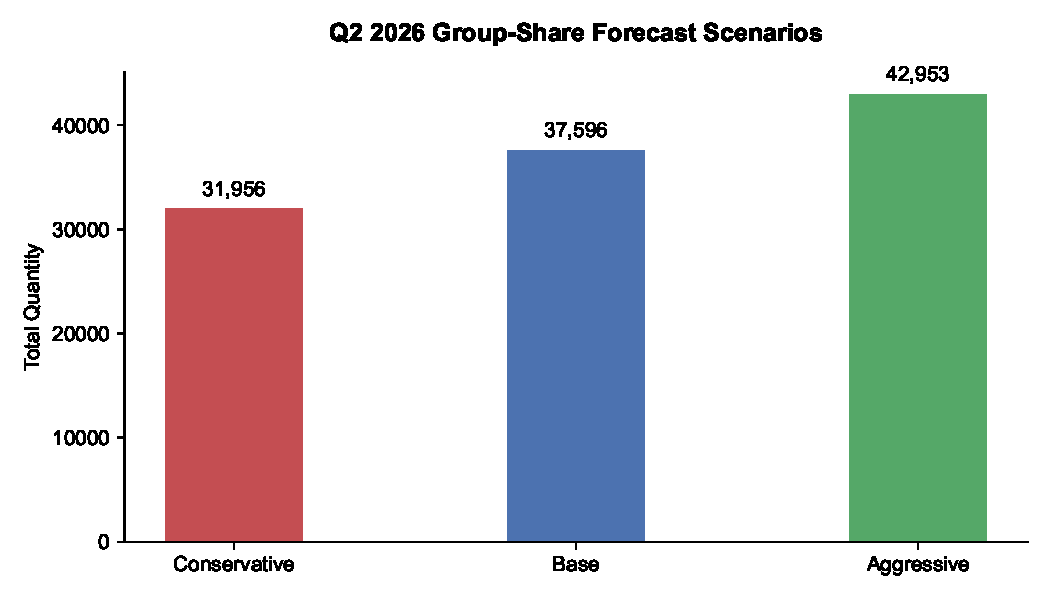
\includegraphics[width=0.85\textwidth]{../figures/en/scenario_forecast.pdf}
\caption{Q2 2026 Group-Share Forecasted Quantity Scenarios}
\label{fig:scenario}
\end{figure}

The Base scenario anchors standard material procurement planning. The Aggressive scenario serves as a strategic capacity buffer for supply chain resilience. Finally, the Conservative scenario assists executive management in controlling cash flow and inventory risks.
\FloatBarrier

\section{Track 2: Color Analysis}
Within the bicycle distribution industry, the base color attribute acts as a useful dealer order signal reflecting localized predictions of end-consumer preferences by dealers. Table \ref{tab:color} and Figure \ref{fig:color} illustrate the Top 10 primary colors dominating the upcoming procurement cycle.

\subsection{Color Contribution and Inventory Implications}
Top colors listed below serve as strong candidates for procurement assurance, heavily driving the bulk of inventory planning. Conversely, low or declining colors require an inventory watch to mitigate stagnant stock. It is crucial to note that this color forecast exclusively reflects a dealer order signal, and should not be perfectly conflated with absolute end-consumer preference.

\begin{table}[H]
\centering
\small
\caption{Top Color Contribution Summary}
\label{tab:color}
\resizebox{\linewidth}{!}{
\begin{tabular}{lllll}
\toprule
\textbf{Color} & \textbf{Forecast Qty} & \textbf{Qty Share} & \textbf{Forecast Rev (VND)} & \textbf{Rev Share} \\
\midrule
Cream & 6,549 & 17.4\% & 10,178,738,540 & 16.7\% \\
Black & 5,797 & 15.4\% & 10,170,423,274 & 16.7\% \\
Gray & 4,308 & 11.5\% & 8,112,828,292 & 13.3\% \\
Pink & 3,816 & 10.1\% & 5,486,401,943 & 9.0\% \\
Green & 3,253 & 8.7\% & 5,418,630,863 & 8.9\% \\
Blue & 3,136 & 8.3\% & 4,786,143,217 & 7.9\% \\
White & 2,857 & 7.6\% & 4,997,821,606 & 8.2\% \\
Brown & 2,018 & 5.4\% & 3,055,462,552 & 5.0\% \\
Mint & 1,968 & 5.2\% & 3,005,926,217 & 4.9\% \\
Red & 1,707 & 4.5\% & 2,520,059,229 & 4.1\% \\
\bottomrule
\end{tabular}
}
\begin{flushleft}
\footnotesize \textit{Note.} Source: outputs/modeling/phase3\_color\_summary\_q2\_2026.csv (columns: Group\_Share\_Base\_Qty, Group\_Share\_Base\_Rev). Forecast revenue is computed from the Group-Share proportional allocation applied to each base color. Qty Share and Rev Share are computed as a percentage of the total Q2 Base scenario forecast (37,596 units / 60,914,780,907 VND).
\end{flushleft}
\end{table}


\begin{figure}[H]
\centering
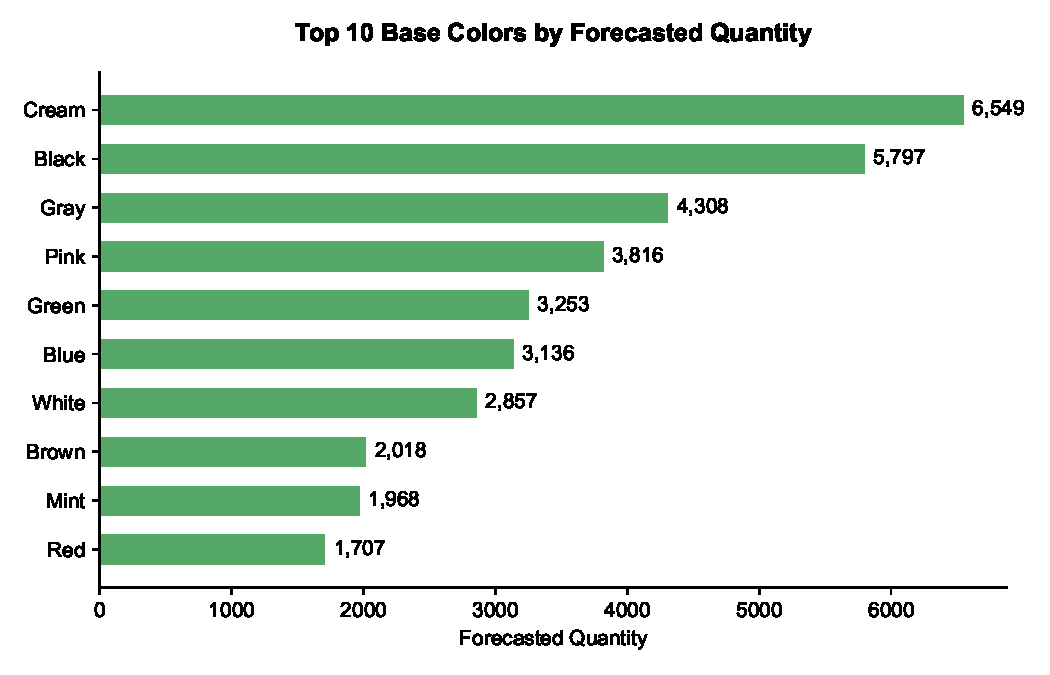
\includegraphics[width=0.85\textwidth]{../figures/en/color_summary.pdf}
\caption{Top 10 Base Colors by Forecasted Quantity (Base Scenario)}
\label{fig:color}
\end{figure}

Colors falling outside this Top 10 tier, or those exhibiting severe historical demand slumps, are systematically flagged as slow-moving SKUs. This automated flagging empowers the sales department to execute early inventory liquidations, phasing out unviable variants before they negatively impact warehouse capacity.
\FloatBarrier

\section{Track 3: Dealer Ranking}
Based on the established RFM B2B (Recency, Frequency, Monetary) paradigm, the system categorized the entire network of 798 dealers into 8 strategic segments. These segments were combined with a risk classification model to establish a unified Priority Ranking.

\subsection{Dealer Segment Value Analysis}
To understand the financial implications of these segments, Table \ref{tab:dealer} and Figure \ref{fig:dealer} describe the monetary distribution across the network. Revenue by dealer segment is directly calculated using available monetary metrics from the RFM processing phase.

\begin{table}[H]
\centering
\small
\caption{Dealer Segment Value Summary}
\label{tab:dealer}
\resizebox{\linewidth}{!}{
\begin{tabular}{llllll}
\toprule
\textbf{Segment} & \textbf{Dealer Count} & \textbf{Historical Revenue (VND)} & \textbf{Revenue Share} & \textbf{Avg Revenue per Dealer (VND)} & \textbf{Avg Priority} \\
\midrule
Champions & 91 & 47,412,839,496 & 43.3\% & 521,020,214 & 64.29 \\
At Risk & 190 & 16,904,146,839 & 15.4\% & 88,969,194 & 21.30 \\
Potential & 184 & 16,412,540,750 & 15.0\% & 89,198,591 & 33.04 \\
Loyal & 47 & 14,744,131,882 & 13.5\% & 313,704,934 & 55.62 \\
Big Spender & 21 & 8,617,826,036 & 7.9\% & 410,372,668 & 38.39 \\
Lost & 215 & 4,407,212,836 & 4.0\% & 20,498,664 & 3.12 \\
Hibernating & 32 & 533,687,109 & 0.5\% & 16,677,722 & 7.10 \\
New & 18 & 412,776,491 & 0.4\% & 22,932,027 & 9.06 \\
\bottomrule
\end{tabular}
}
\begin{flushleft}
\footnotesize \textit{Note.} Source: outputs/modeling/phase3\_dealer\_priority\_ranking\_q2\_2026.csv. Segment monetary totals reconcile to the historical revenue total of 109,445,161,439 VND.
\end{flushleft}
\end{table}


\begin{figure}[H]
\centering
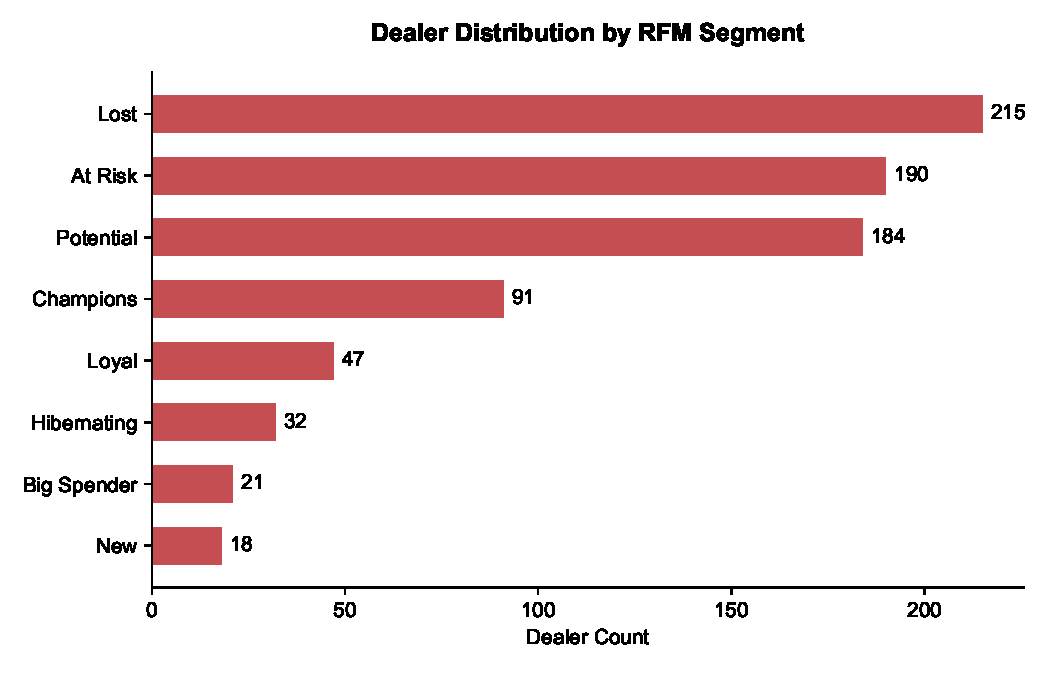
\includegraphics[width=0.85\textwidth]{../figures/en/dealer_segmentation.pdf}
\caption{Dealer Distribution by RFM Segment}
\label{fig:dealer}
\end{figure}

The Champions and Loyal segments act as the primary, stable revenue drivers. The Big Spender demographic requires a dedicated Key Account Care approach, as their purchasing patterns are voluminous but infrequent. Forcing aggressive sales frequency upon this group could prove counterproductive. Conversely, the high volume of Lost and At Risk accounts necessitates immediate reactivation campaigns.

\subsection{Strategic Action Matrix}
To translate these insights into actionable business strategies, Table \ref{tab:dealer_matrix} outlines the recommended approaches and Key Performance Indicators (KPIs) to monitor for each primary segment.

\begin{table}[H]
\centering
\small
\caption{Dealer Action Matrix}
\label{tab:dealer_matrix}
\resizebox{\linewidth}{!}{
\begin{tabular}{lllll}
\toprule
\textbf{Segment} & \textbf{Business Meaning} & \textbf{Risk} & \textbf{Recommended Action} & \textbf{KPI to Monitor} \\
\midrule
Champions & High value, frequent & Low & Retain and protect & Retention rate / Repeat revenue \\
Loyal & Steady buyers & Low & Maintain engagement & Order frequency \\
Big Spender & High value, rare & Medium & Dedicated account care & Total revenue / Account retention \\
Potential & Promising buyers & Medium & Nurture and convert & Conversion to Loyal/Champion \\
At Risk & Dropping frequency & High & Reactivation campaign & Reactivation rate \\
Lost & Inactive long term & Very High & Low-cost reactivation or deprioritize & Response rate \\
Hibernating & Inactive & High & Periodic nurture & Reactivation signal \\
New & Just onboarded & Unknown & Onboarding & Second order rate \\
\bottomrule
\end{tabular}
}
\begin{flushleft}
\footnotesize \textit{Note.} Strategic actions and KPIs tailored to each RFM B2B segment.
\end{flushleft}
\end{table}

\FloatBarrier

\section{Dashboard and Deliverables}
All analytical pipelines converge into final output Artifacts designed for immediate business consumption. Table \ref{tab:artifacts} outlines which artifacts are designated for various stakeholder groups.

\begin{table}[H]
\centering
\small
\caption{Which Artifact Should Each Stakeholder Use?}
\label{tab:artifacts}
\resizebox{\linewidth}{!}{
\begin{tabular}{lll}
\toprule
\textbf{Stakeholder} & \textbf{Primary Need} & \textbf{Recommended Artifacts} \\
\midrule
Executive Team & Strategic overview & Executive Summary, Scenario Delta Table \\
Supply Chain / Procurement & Volume planning & Group-Share Forecast, Color Forecast \\
Sales / Trade Marketing & Dealer prioritization & Dealer Priority Ranking, Action Matrix \\
Data Science & Model stability & Feature Importance, ML Model Comparison \\
\bottomrule
\end{tabular}
}
\begin{flushleft}
\footnotesize \textit{Note.} Maps final outputs to specific operational workflows.
\end{flushleft}
\end{table}


For BI visualization, the system architecture connects Power BI directly into the data warehouse via optimized views such as \texttt{v-rfm-analysis}. This ensures dashboards reflect real-time analytical updates.
\FloatBarrier

\section{Pipeline Reproducibility}
Pipeline reproducibility ensures that historical validations can be re-run consistently. The Python architecture operates purely via CLI arguments to enforce immutable rules. Raw CSVs, interim data, feature stores, cache files, and model binaries are intentionally excluded from version control; the pipeline runner regenerates derived artifacts locally.

\begin{lstlisting}[language=bash]
# 1. Dry-run to validate pipeline structure without overwriting
python src/models/forecasting/run_end_to_end.py --dry-run

# 2. End-to-End execution
python src/models/forecasting/run_end_to_end.py --allow-modeling --allow-overwrite
\end{lstlisting}
\FloatBarrier

\section{Limitations and Future Work}
While providing a stable operational baseline, the system carries fundamental technical limitations that dictate clear avenues for future enhancement:
\begin{itemize}
    \item \textbf{Short History}: The absence of 9 core months of data in 2025 severely restricts cyclical analysis, requiring additional real historical data or carefully documented scenario assumptions in future iterations.
    \item \textbf{March Shock}: The sudden demand surge may incite overfitting phenomena in short-term forecasting if tree weights are not heavily regularized.
    \item \textbf{Cold-start Problem}: Newly onboarded dealers lack sufficient transactional history, inhibiting the generation of meaningful RFM behavioral scores.
    \item \textbf{Probability Calibration}: The Track 3 Classifier currently emits uncalibrated probabilities. Integrating Isotonic Regression or Platt Scaling is necessary to improve churn risk reliability.
\end{itemize}
\FloatBarrier


\end{document}
